%%%%%%%%%%%%%%%%%%%%%%%%%%%%%%%%%%%%%%%%%
% Stylish Curriculum Vitae
% LaTeX Template
% Version 1.1 (September 10, 2021)
%
% This template originates from:
% https://www.LaTeXTemplates.com
%
% Authors:
% Stefano (https://www.kindoblue.nl)
% Vel (vel@LaTeXTemplates.com)
%
% License:
% CC BY-NC-SA 4.0 (https://creativecommons.org/licenses/by-nc-sa/4.0/)
%
%%%%%%%%%%%%%%%%%%%%%%%%%%%%%%%%%%%%%%%%%
% !TEX program = xelatex
\documentclass[a4paper, oneside, final, 12pt]{scrartcl} % Paper options using the scrartcl class

\usepackage{fontspec} % for other font
\usepackage{xeCJK} % for chinese font
\usepackage{hyperref} % for hyper web link
\usepackage{multirow} % for tabular table in learning progress
\usepackage{graphicx} % for image insersion
\usepackage[export]{adjustbox} % for image frame
\usepackage{setspace}
\usepackage{array}
% Define typographic struts, as suggested by Claudio Beccari
%   in an article in TeX and TUG News, Vol. 2, 1993.
\usepackage{mathptmx}
\usepackage{scrlayer-scrpage} % Provides headers and footers configuration
\usepackage{titlesec} % Allows creating custom \section's
\usepackage{marvosym} % Allows the use of symbols
\usepackage{tabularx,colortbl} % Advanced table configurations
% \usepackage{ebgaramond} % Use the EB Garamond font
\usepackage{microtype} % To enable letterspacing
\usepackage{pdfpages} % for showing pdf
\usepackage{pdflscape}
\usepackage{enumitem}
\usepackage{subcaption}
\usepackage{listings}   % highlight the python code
\usepackage{xcolor}
\usepackage{multirow}
\usepackage{cite} %Imports biblatex package
\usepackage[ruled,linesnumbered]{algorithm2e}
\newcommand\mycommfont[1]{\normalsize\ttfamily\textcolor{blue}{#1}}
\SetCommentSty{mycommfont}
% \usepackage[backend=bibtex,bibencoding=ascii,style=authoryear,sorting=none]{bibtex}
% \addbibresource{reference.bib}
% setup the margin
\usepackage[top=1cm, bottom=1cm, right=2cm, left=2cm]{geometry}

% set the style of listing code
\definecolor{codegreen}{rgb}{0,0.6,0}
\definecolor{codegray}{rgb}{0.5,0.5,0.5}
\definecolor{codepurple}{rgb}{0.58,0,0.82}
\definecolor{backcolour}{rgb}{0.95,0.95,0.92}

\lstdefinestyle{mystyle}{
    backgroundcolor=\color{backcolour},   
    commentstyle=\color{codegreen},
    keywordstyle=\color{magenta},
    numberstyle=\tiny\color{codegray},
    stringstyle=\color{codepurple},
    basicstyle=\ttfamily\footnotesize,
    breakatwhitespace=true,         
    breaklines=true,                 
    captionpos=b,                    
    keepspaces=true,                 
    numbers=left,                    
    numbersep=5pt,                  
    showspaces=false,                
    showstringspaces=false,
    showtabs=false,                  
    tabsize=2
}

\lstset{style=mystyle}

% set chinese and english font
\setmainfont{Times New Roman}
\setCJKmainfont[AutoFakeBold=true, AutoFakeSlant=true]{標楷體}

\titleformat{\section}{\Large\raggedright\bfseries}{}{0em}{}[\titlerule] % Section formatting
\titleformat{\subsection}{\large\raggedright\bfseries}{}{0em}{}
\titleformat{\subsubsection}{\normalsize\raggedright\bfseries}{}{0em}{}

% \pagestyle{scrheadings} % Print the headers and footers on all pages

% enable bold and slant chinese font
% \xeCJKsetup{AutoFakeBold=true, AutoFakeSlant=true}

% set the space at the front of paragraph
\setlength{\parindent}{2em}

% disable page number
\pagenumbering{gobble}

\newcommand{\gray}{\rowcolor[gray]{.90}} % Custom highlighting for the work experience and education sections
\newcommand{\Tstrut}{\rule{0pt}{2.6ex}}         % = `top' strut
\newcommand{\Bstrut}{\rule[-0.9ex]{0pt}{0pt}}   % = `bottom' strut
\newcommand{\Tstruth}{\rule{0pt}{4ex}}         % = `top' strut for header
\newcommand{\Bstruth}{\rule[-2.5ex]{0pt}{0pt}}   % = `bottom' strut for header

%----------------------------------------------------------------------------------------
%	FOOTER SECTION
%----------------------------------------------------------------------------------------

% \renewcommand{\headfont}{\normalfont\rmfamily\scshape} % Font settings for footer

% \cofoot{
% \fontsize{12.5}{17}\selectfont % Letter spacing and font size

% \textls[150]{123 Broadway {\large\textperiodcentered} City {\large\textperiodcentered} Country 12345}\\ % Your mailing address
% {\Large\Letter} \textls[150]{john@smith.com \ {\Large\Telefon} (000) 111-1111} % Your email address and phone number
% }

%----------------------------------------------------------------------------------------
\begin{document}

%----------------------------------------------------------------------------------------
%	HEADER SECTION
%----------------------------------------------------------------------------------------


\begin{center}
    {\fontsize{18}{30}\textbf{NYCU 2023 Autumn \\ Data Vislualization \\ Final Project Proposal Team23}} \\
\end{center}

% list two authors information side by side
  \begin{minipage}[t]{0.45\textwidth}
    \begin{center}
      \textbf{Bo-Han Chen (陳柏翰)} \\
      Student ID: 312551074 \\
      bhchen312551074.cs12@nycu.edu.tw
    \end{center}
  \end{minipage}
  \begin{minipage}[t]{0.45\textwidth}
    \begin{center}
      \textbf{Xu Lin (林煦)} \\
      Student ID: 312553027 \\
      f94061042.cs12@nycu.edu.tw
    \end{center}
  \end{minipage}

\section{Dataset}

\begingroup
\raggedright

The dataset we choose is the Taiwan road traffic accident statistics 
in 2022 (\emph{111年傷亡道路交通事故資料}), which contains the details of
the accidents that cause death or injury in Taiwan.
The dataset is public and can be accessed from Open Data Website of Taiwan Government
\footnote{\url{https://data.gov.tw/dataset/161199}.}.

\subsection{Data Description}

The dataset contains 845547 records, 
including 4544 A1 level records and 841003 A2 records.
The A1 level means the accident causes death in within 24 hours,
and the A2 level means the accident causes injury or death in more than 24 hours.
Each record contains 51 attributes, including the time, location,
weather, road type, vehicle type, and the number of death/injury.
Some details such as whether the driver is drunk or not, 
which part of the vehicle hit in the accident, 
and the driver-contributed cause of the accident are also included.

\section{Motivation}

Since there are many people injured or killed in traffic accidents every year,
so the analysis of the traffic accident data 
is important and necessary to prevent the accident.
Some of the accidents are caused by the driver's behavior,
and some are caused by the road condition 
and the circumstance such as weather condition at the time that the accident happened.
Therefore, an easy-to-understand data vislualization 
can help the experts to analyze the cause of the accident
and promote the right policy to drivers and pedestrians.
By analyzing the circumstance of the accident,
we can also find the dangerous road condition and time period,
which can help the government to decrease the accident rate 
by improving the road condition and employing more traffic police at the certain time period.

\subsection{Questions to Answer}

The following questions are what we want to answer by visualizing the dataset.

\begin{enumerate}
  \item Which time period has the highest accident rate?
  \item Which weather condition mainly causes the accident?
  \item Is there any relationship between the 
  driver-contributed causes and the type of vehicle?
  \item Which part of the vehicle is most likely to be hit and fragile during the crash?
\end{enumerate}

\section{Methodology}

The overview of our visualization system is shown in Figure \ref{fig:overview_part}.

\begin{figure}[t]
  \centering
  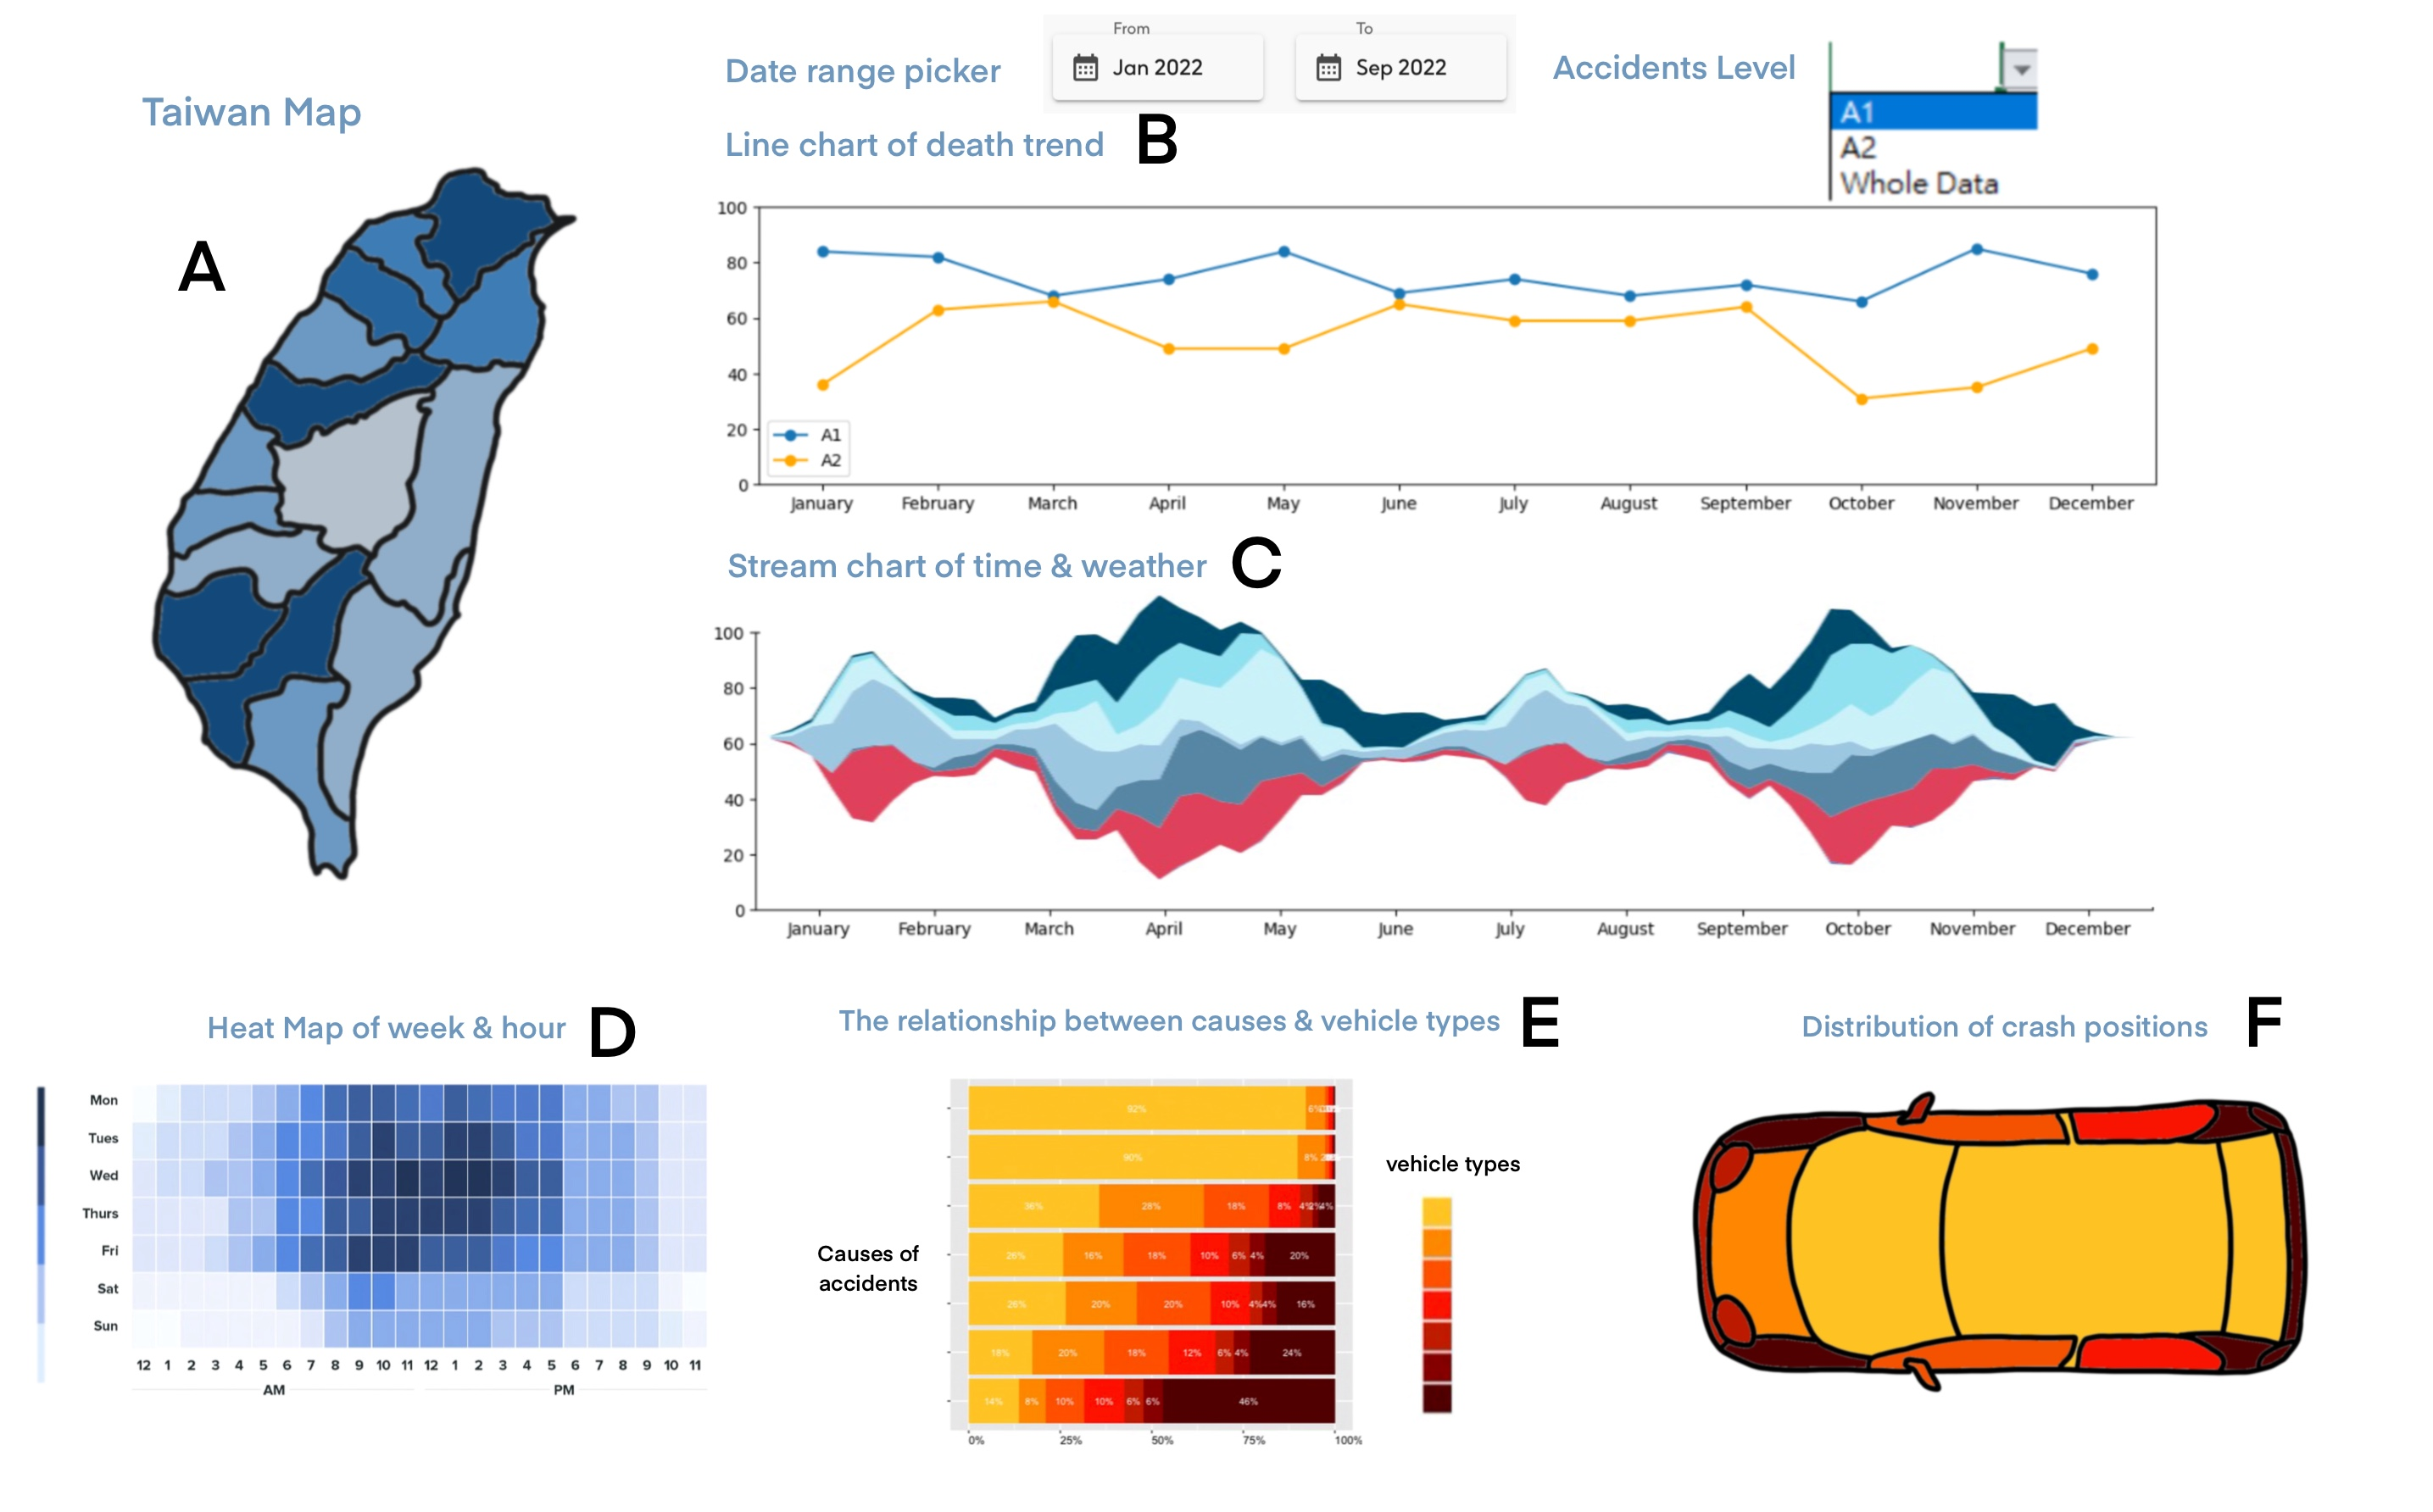
\includegraphics[width=\textwidth]{Image/overview_part.jpg}
  \caption{Overview of our visualization system}
  \label{fig:overview_part}
\end{figure}

\subsection{Taiwan Car Crash Accident Map}

The map (\textbf{part A}) shows the number of accident in each city
by heatmap, with darker color means higher accident rate.
The user can move the mouse to the city to see the statistics details
such as the ratio of drunk driving and mobile phone usage.

\subsection{Accident Statistics Over Time}

The line chart (\textbf{part B}) is used to let user discover the trend of the accident occurence
over months and years. And user can also select and focus on specific time period.
However, it's not enough to depicts the trend of accidents 
from the perspective of months and years.
So we also use the grid heatmap (\textbf{part D}) to represent 
the accident occurence by time of day and day of week.
We expect it can provide another detailed view of traffic accident trend.

\subsection{Weather Condition}

The stream chart (\textbf{part C}) is used to show the trend of the accident with different weather condition.
With this chart, we expect to find the weather-related cause of the accident in certain time period.
For example, there might have more accident caused by rainy day in monsoon or typhoon season.

\subsection{Vehicle and Driver Information}

The stacked bar chart (\textbf{part E}) is used to show the relationship between the driver-contributed causes
and the type of vehicle. With this chart, we can find the frequent cause of the accident
and the type of vehicle that corresponds to the cause. \\

The car chart (\textbf{part F}) shows the distribution of crash positions of the vehicle.
With this chart, we can find the frequent crash position of the vehicle
and the crash part that causes more death with A1 level data.

% \subsection{Color Selection}

% For cartography color selection, 
% we use the colorbrewer2\footnote{\url{https://colorbrewer2.org/}.}
% to select the color scheme for our map.
% For ordered data, we choose the viridis color scheme,
% which is colorblind-friendly and perceptually uniform.

\endgroup

% \bibliographystyle{unsrt} % We choose the "plain" reference style
% \bibliography{reference} % Entries are in the "references.bib" file

\end{document}